\section{ugetpid.c}
Trong hệ điều hành xv6, bình thường khi một tiến trình gọi
\code{getpid()}, chương trình phải thực hiện lệnh \code{ecall} để bẫy
vào kernel, lưu các thanh ghi vào \code{TRAPFRAME}, đổi bảng trang
sang kernel rồi mới đọc giá trị PID và quay lại user mode bằng
\code{sret} \cite{xv6book}. Để tiết kiệm chi phí chuyển qua lại này
cho những thông tin chỉ đọc, bài lab yêu cầu chia sẻ một trang nhớ chỉ
đọc giữa kernel và tiến trình user tại địa chỉ ảo cố định
\code{USYSCALL}, giúp hàm \code{ugetpid()} đọc thẳng PID ngay ở không
gian người dùng \cite{hcmus_os_lab3,mitpgtbl}.

\subsection{Triển khai}
Để triển khai được tính năng này, trước tiên ta cần định nghĩa địa chỉ
ảo \code{USYSCALL} trong file \texttt{kernel/memlayout.h} với giá trị
bằng \code{TRAPFRAME - PGSIZE}, tức là nằm thấp hơn \code{TRAPFRAME}
đúng một trang $4096$ byte. Tiếp theo, nhóm tạo file
\texttt{kernel/usyscall.h} để định nghĩa cấu trúc
\code{struct usyscall} gồm một trường \code{int pid}, kèm theo
\texttt{\#ifndef XV6\_USYSCALL\_H} để tránh lỗi khai báo trùng khi nạp
ở cả phía kernel lẫn user. Trong \code{struct proc} của file
\texttt{kernel/proc.h}, ta thêm con trỏ \code{struct usyscall
*usyscall} để mỗi tiến trình trỏ tới trang chia sẻ của riêng mình
\cite{xv6vm}.

Khi một tiến trình mới được tạo trong hàm \code{allocproc()} tại
\texttt{kernel/proc.c}, sau khi đã cấp PID và trang \code{trapframe},
ta gọi \code{kalloc()} để xin một trang vật lý cho \code{p->usyscall}.
Nếu thiếu RAM và \code{kalloc()} trả về $0$, hàm sẽ gọi
\code{freeproc(p)} để dọn tài nguyên đã cấp trước đó, nhả khóa
\code{release(\&p->lock)} rồi trả về $0$. Khi cấp được trang mới, ta
dùng \code{memset()} xóa sạch cả $4096$ byte để không bị sót dữ liệu
cũ của kernel, rồi gán \code{p->usyscall->pid = p->pid}.

\paragraph*{Ánh xạ và thu hồi:} Sau khi đã có trang vật lý ở trên,
bước tiếp theo là gắn nó vào bảng trang của tiến trình trong hàm
\code{proc\_pagetable()}. Ngay dưới đoạn ánh xạ \code{TRAMPOLINE} và
\code{TRAPFRAME}, ta gọi \code{mappages()} để nối địa chỉ ảo
\code{USYSCALL} kích thước \code{PGSIZE} tới \code{(uint64)p->usyscall}
với quyền \code{PTE\_R | PTE\_U}. Ta chỉ bật quyền đọc cho user mà không
bật \code{PTE\_W} để chương trình người dùng đọc được PID chứ không tự
sửa được. Nếu \code{mappages()} thất bại, ta dùng \code{uvmunmap()} gỡ
lại hai ánh xạ \code{TRAPFRAME} và \code{TRAMPOLINE} với
\code{do\_free = 0} rồi gọi \code{uvmfree(pagetable, 0)} tương tự như
đoạn xử lý lỗi ngay phía trên trong file \texttt{kernel/proc.c}.

Khi tiến trình kết thúc và gọi \code{proc\_freepagetable()}, ta phải
chạy \code{uvmunmap()} cho \code{USYSCALL} với $1$ trang và
\code{do\_free = 0} trước khi gọi \code{uvmfree(pagetable, sz)}. Lý do
là hàm \code{freewalk()} bên trong \code{uvmfree()} yêu cầu mọi trang
lá phải được gỡ ánh xạ trước, nếu quên bước này thì kernel sẽ bị
\code{panic("freewalk: leaf")}. Còn tham số \code{do\_free} để bằng $0$
vì trang RAM của \code{p->usyscall} sẽ được giải phóng bằng
\code{kfree()} bên trong \code{freeproc()} rồi đặt con trỏ về $0$.

\paragraph*{Hàm đọc nhanh ở user và câu hỏi mở rộng:} Ở phía người
dùng, nhóm khai báo hàm \code{int ugetpid(void);} trong file
\texttt{user/user.h} và viết phần thân trong \texttt{user/ulib.c}.
Trong \code{ugetpid()}, ta chỉ cần ép địa chỉ \code{USYSCALL} sang
\code{struct usyscall *} rồi trả về giá trị trường \code{pid}. Vì
trang này đã được map sẵn với quyền đọc cho user nên CPU đọc thẳng từ
bộ nhớ mà không cần chạy qua \code{ecall}.

Theo câu hỏi thêm của đề bài \cite{hcmus_os_lab3}, những system call
khác trong xv6 chỉ đọc dữ liệu có sẵn mà không làm thay đổi trạng thái
của kernel cũng có thể tăng tốc bằng trang chia sẻ này. Ví dụ như
\code{getppid()} nếu ta lưu thêm trường \code{ppid} vào
\code{struct usyscall} và cập nhật lại khi \code{fork()} hay khi cha
thoát; hoặc \code{uptime()} nếu kernel chia sẻ chung một trang chỉ đọc
chứa biến đếm \code{ticks}; hay việc đọc kích thước bộ nhớ \code{p->sz}
khi được kernel đồng bộ mỗi lần \code{exec()} hoặc \code{sbrk()} chạy.

Sơ đồ dưới đây tóm tắt luồng ánh xạ trang \code{USYSCALL} và cách
\code{ugetpid()} đọc trực tiếp PID từ không gian người dùng mà không cần
chuyển ngữ cảnh vào kernel:

\begin{figure}[H]
  \centering
  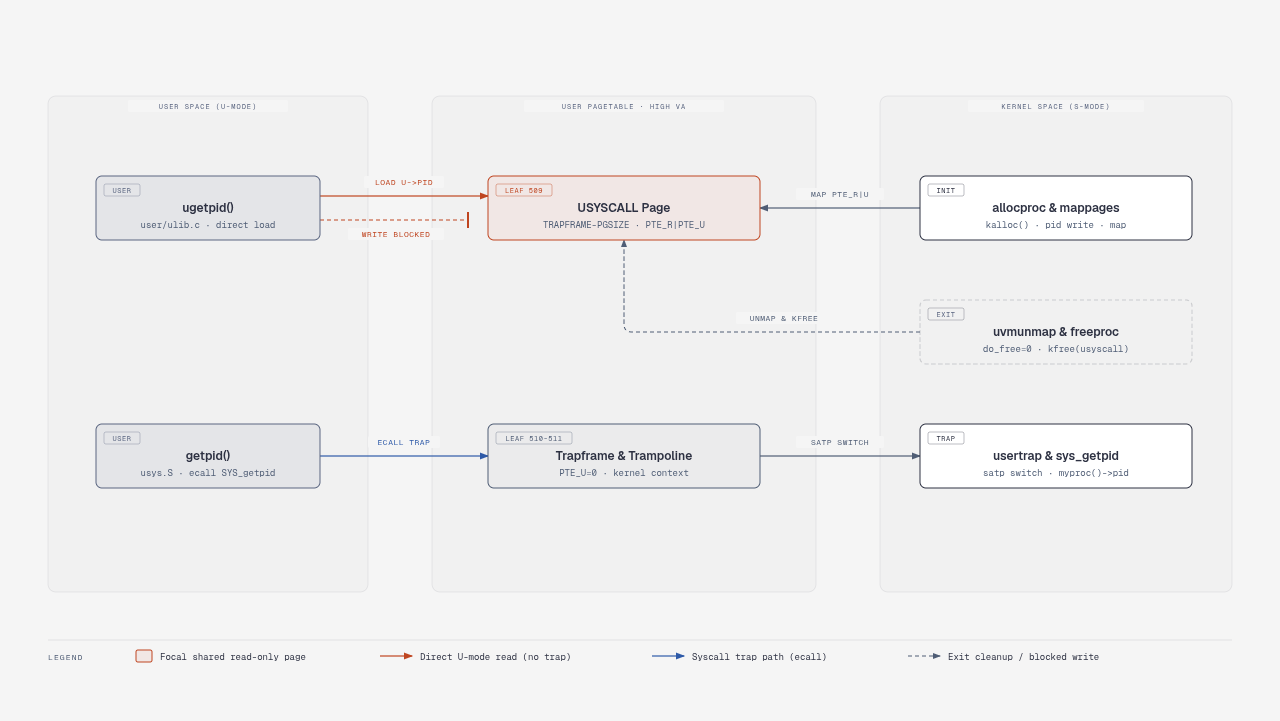
\includegraphics[width=\linewidth]{images/usyscall_arch.png}
  \caption{Kiến trúc ánh xạ trang \code{USYSCALL} và đường đi của
  \code{ugetpid()}}
  \label{fig:usyscall_arch}
\end{figure}

\subsection{Kiểm thử}
Để kiểm tra việc ánh xạ \code{USYSCALL} và hàm \code{ugetpid()}, nhóm
tạo file \texttt{user/ugetpidtest.c} và thêm vào \code{UPROGS} trong
\texttt{Makefile} nhằm đối chiếu trực tiếp kết quả giữa \code{getpid()}
và \code{ugetpid()} (Bảng~\ref{tab:ugetpid_checks}).

\begin{table}[H]
    \centering
    \small
    \renewcommand{\arraystretch}{1.25}
    \begin{tabularx}{\textwidth}{p{0.35\textwidth} X}
        \toprule
        \textbf{Trường hợp kiểm tra} &
        \textbf{Mục đích kiểm tra} \\
        \midrule
        \texttt{ugetpidtest} &
        So sánh trực tiếp giá trị trả về của \code{getpid()} và
        \code{ugetpid()} trên tiến trình đang chạy. \\
        Đối chiếu bảng trang của \texttt{init} qua \code{vmprint} &
        Kiểm tra mục L0 chỉ số $509$ tại \code{USYSCALL} có đúng cờ
        quyền \code{0x13} (\code{PTE\_V | PTE\_R | PTE\_U}) hay không. \\
        \bottomrule
    \end{tabularx}
    \caption{Các trường hợp kiểm tra tính năng \texttt{ugetpid}}
    \label{tab:ugetpid_checks}
\end{table}

Khi chạy thực tế trên QEMU, chương trình \texttt{ugetpidtest} in ra
hai giá trị PID trùng khớp nhau và thoát bình thường:
\begin{lstlisting}[style=terminalstyle]
$ ugetpidtest
getpid()  = 3
ugetpid() = 3
PID matched: 3
\end{lstlisting}
